\newcommand{\RM}[1]{\MakeUppercase{\romannumeral #1{}}}

\chapter{Tunneldiode\label{chapter:tunneldiode}}
\lhead{Tunneldiode}
\begin{refsection}
\chapterauthor{Stefan Hedinger}

\newpage
\section{Einleitung}
\rhead{Einleitung}
Die Tunneldiode ist ein nicht sehr h"aufig verwendetes, aktives und dynamisches Halbleiterelement. Die beiden Seiten des p-n-"Ubergangs sind stark dotiert. Durch den besonderen Aufbau und die starke Dotierung k"onnen Elektronen die Sperrschicht passieren bevor die Diode leitet.

Sie hat eine spezielle Kennlinie, welche im mittleren Bereich einen negativen Widerstand aufweist.

\begin{figure}[h]	%Bild Kennlinie der Tunneldiode
\centering
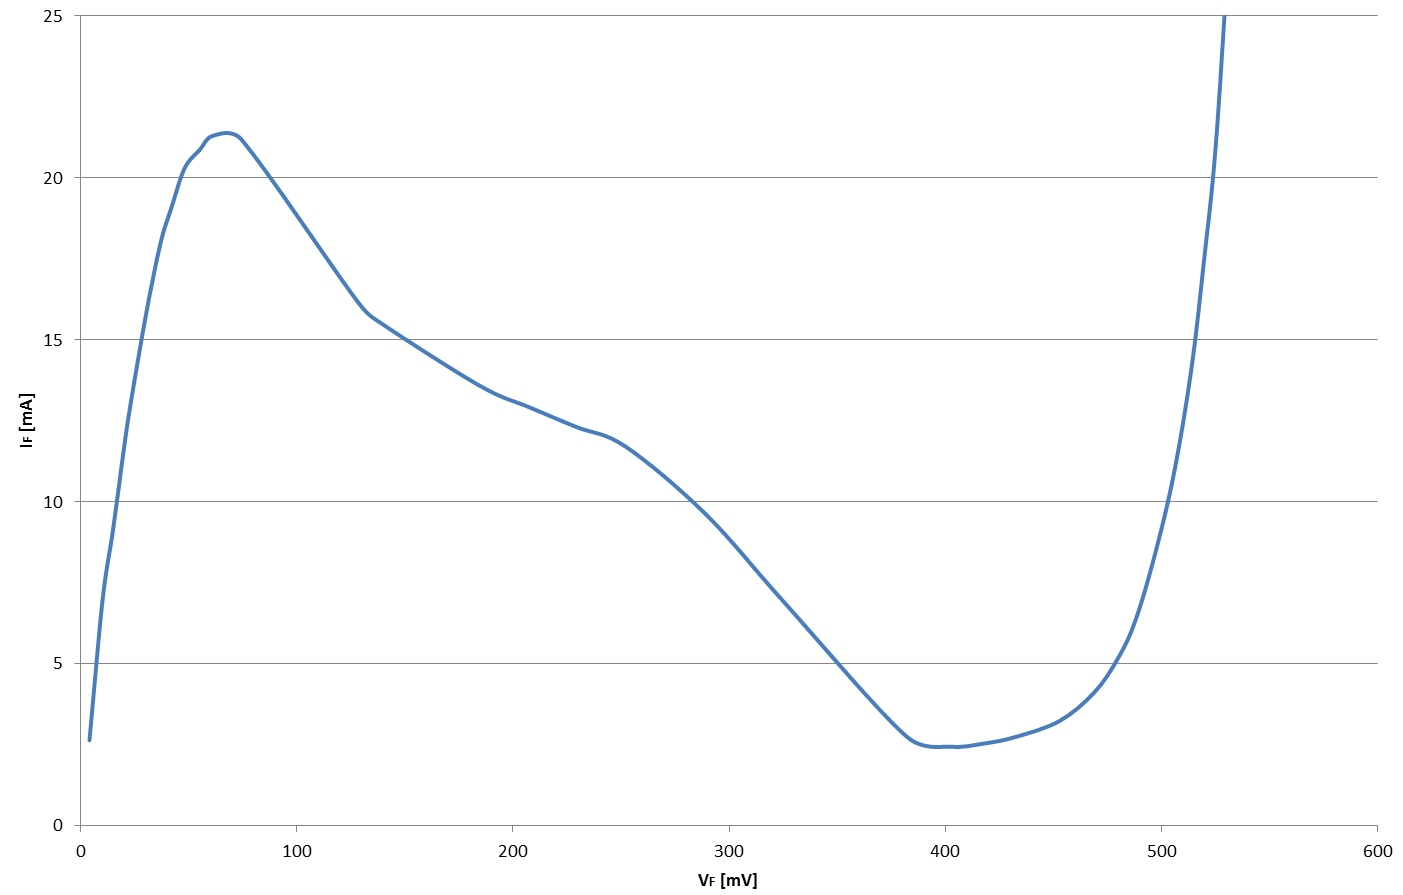
\includegraphics[width=0.7\textwidth]{tunneldiode/images/Tunneldiode.png}
\caption{Die spezielle Kennlinie der Tunneldiode
\label{skript:Tunneldiode}}
\end{figure}

\section{Tunneleffekt}
\rhead{Tunneleffekt}
Die Vorg"ange in der Tunneldiode werden mit dem Tunneleffekt beschrieben. Zum besseren Verst"andnis betrachten wir das Potential 
\[
V(x)=\begin{cases}
V_0& \qquad \text{wenn } x \in [-a,a]\\
0&   \qquad \text{sonst}
\end{cases}
\]
in den verschiedenen Bereichen.

Ein Teilchen kommt von links und m"ochte nach rechts. Die Energie vom einfallenden Teilchen ist $E$ und es gilt
\[
0 < E < V_0.
\]
In der Mitte ist aber eine Barriere, welche ein h"oheres Potential als das Teilchen selber aufweist. In der normalen Mechanik ist klar, dass dieses Teilchen nicht von links nach rechts kommt sondern an der Barriere bei -a reflektiert wird. In der Quantenmechanik k"onnen Teilchen jedoch durch die Barriere durchtunneln.

\begin{figure}[h]	%Bild Kastenpotential
\centering
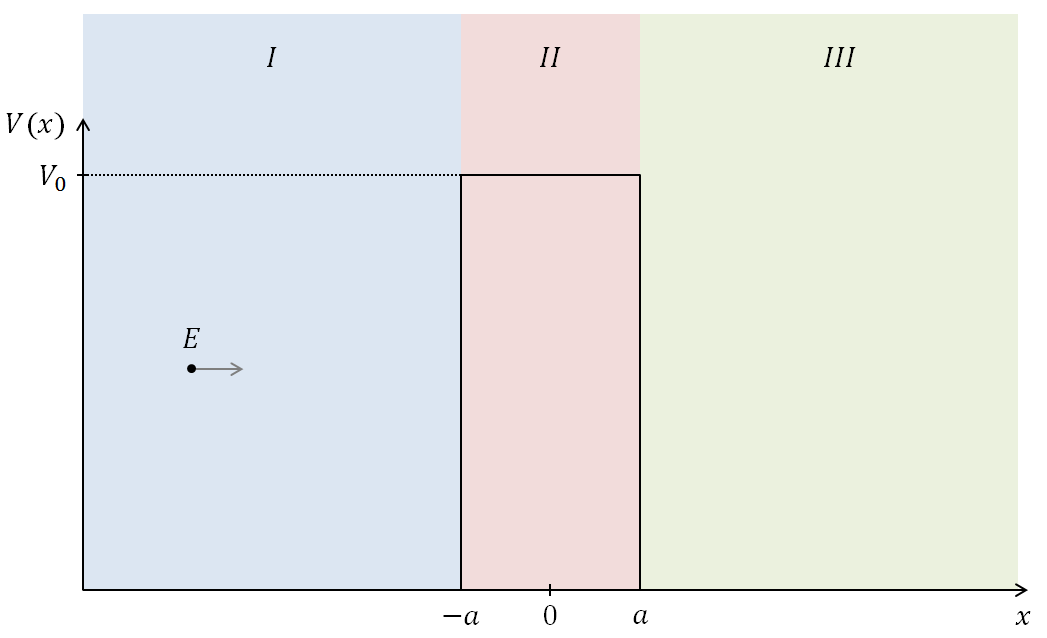
\includegraphics[width=0.7\textwidth]{tunneldiode/images/Kastenpotential.png}
\caption{Kastenpotential
\label{skript:Kastenpotential}}
\end{figure}

Die nachfolgenden Berechnungen sollen helfen, den Tunneleffekt zu verstehen.  Als erstes betrachten wir die statin"are Schr"odingergleichung f"ur die Wellenfunktion $\Phi(x)$. Dabei ist $m$ die Masse und $E$ die Energie des Teilchens.
\[
E\Phi(x) = -\frac{\hbar^2}{2m}\frac{d^2}{dx^2}\Phi(x) + V(x)\Phi(x)
\]
Im Bereich \RM{1} und \RM{3} verwenden wir f"ur die Wellenfunktion den allgemeine Ansatz
\[
\Phi(x) = Ae^{ikx}+Be^{-ikx}.
\]
F"ur $k$ gilt dabei
\[
k = \sqrt{\frac{2mE}{\hbar^2}}.
\]
Abgeleitet vom allgemeinen Ansatz m"ussen jetzt nur noch $A$ und $B$ bestimmt werden. Im Bereich \RM{1} ist
\[
A = 1 \text{ und } B = R
\]
da $A$ der Koeffizient der einlaufenden Welle ist und dieser Betragsm"assig als 1 angenommen wird. Diese Annahme ist notwendig, da sich die genaue Anzahl der Teilchen nicht ermitteln l"asst. $B$ ist der Koeffizient der auslaufende Welle. Das $R$ steht somit f"ur die Anzahl reflektierter Teilchen. Somit vereinfacht sich die Gleichung im Bereich \RM{1} zu
\[
\Phi_\RM{1}(x) = e^{ikx} + Re^{-ikx}.
\]

Im Bereich \RM{3} gilt
\[
A = T \text{ und } B = 0.
\]
Auch hier ist $A$ der Koeffizient der einlaufenden Welle und damit der transmittierten Teilchen, also $T$. Die m"oglicherweise in diesem Bereich reflektierten Teilchen interessieren uns nicht. Deshalb setzen wir $B$ auf 0. Somit erhalten wir f"ur den Bereich \RM{3} die Gleichung
\[
\Phi_\RM{3}(x) = Te^{ikx}.
\]
F"ur die Wellenfunktion im Bereich \RM{2} lautet die Gleichung
\[
\Phi_\RM{2}(x) = \alpha e^{\kappa x} + \beta e^{-\kappa x}
\]
da wir in der Potentialbarriere einen exponentiellen Abfall oder Anstieg erwarten. $\kappa$ ist
\[
\kappa = \sqrt{\frac{2m}{\hbar^2}(V_0 - E)}.
\]
Damit wir die vier Unbekannten $\alpha$, $\beta$, $R$ und $T$ bestimmen k"onnen, m"ussen wir Gemeinsamkeiten der Wellenfunktionen an den "Ubergangsstellen zwischen den Bereichen ausnutzen. Damit die Wellenfunktion ohne Spr"unge zusammengesetzt werden kann muss
\[
\Phi_\RM{1}(-a) = \Phi_\RM{2}(-a)
\]
\[
\Phi_\RM{2}(a) = \Phi_\RM{3}(a)
\]
\[
\Phi_\RM{1}'(-a) = \Phi_\RM{2}'(-a)
\]
\[
\Phi_\RM{2}'(a) = \Phi_\RM{3}'(a)
\]
gelten. Somit haben wir ein Gleichungssystem mit vier Gleichungen f"ur vier Unbekannte. Wir brauchen also die Ableitungen der Wellenfunktionen in den drei Bereichen.
\[
\Phi_\RM{1}'(x) = ike^{ikx} - Rike^{-ikx}
\]
\[
\Phi_\RM{2}'(x) = \alpha \kappa e^{\kappa x} - \beta \kappa e^{-\kappa x}
\]
\[
\Phi_\RM{3}'(x) = Tike^{ikx}
\]


%TODO: Überleitung zur Berechnung mit Matrizen
%      geometrischer Aufbau der Tunneldiode vs. Siliziumdiode
%	   Rückkehr zur Tunneldiode -> Wie der Tunneleffekt da auftritt
\input tunneldiode/t.tex


\printbibliography[heading=subbibliography]
\end{refsection}

